\documentclass[12pt,a4paper]{article}
\usepackage{geometry, graphicx}
\usepackage{geometry, graphicx, float}
\geometry{margin=1in}

\title{SCS 2312 - Compiler Assignment }
\author{A.V.A.R.L.Premathilaka - 23001496}

\begin{document}

\maketitle
\tableofcontents
\newpage

\section{Introduction}
Main goal for this assignment was to design a compiler that represents a real world compiler as closely as possible. The main components and workflow of the compiler is as follows:
\begin{itemize}
    \item \textbf{Lexer} - Takes the input file and produces a stream of tokens
    \item \textbf{Parser} - Takes the stream of tokens and produces a parse tree
    \item \textbf{Executor} - Takes that parse tree and executes the program using a symbol table
\end{itemize}

\section{Grammar Definition}
The grammar below are defined in the syntax of ANTLR4

\subsection{Lexer Grammar}
\begin{verbatim}

STMT_END    :   ';' ;
KW_INT      :   'int' ;
ADD_OP      :   '+' ;
ASSIGN      :   '=' ;

ID          :   [a-zA-Z_][a-zA-Z_0-9]* ;
INT_LITERAL :   [0-9]+ ;

L_PAREN     :   '(' ;
R_PAREN     :   ')' ;

WS          :   [\r\n \t]+ -> skip ;
\end{verbatim}

\subsection{Parser Grammar}
\begin{verbatim}
prog        :   stmt_list ;

stmt_list   :   stmt 
            |   stmt_list stmt
            ;

stmt        :   funcCall 
            |   declaration 
            ;

declaration :   type ID ASSIGN expr STMT_END
            ;

funcCall    :   ID L_PAREN args R_PAREN STMT_END
            |   ID L_PAREN R_PAREN STMT_END
            ;

args        :   term
            ;

term        :   literal 
            |   ID
            ;

literal     :   INT_LITERAL 
            ;
    
type        :   KW_INT
            ;

expr        :   term
            |   expr ADD_OP term
            ;
\end{verbatim}

\section{Code Explanation}
\subsection{Lexer}
\subsubsection{The Lexer DFA}
Here we have implemented the lexer using an actual DFA in the file (\texttt{lexerDFA.c}).
The State diagram for the DFA is as shown below:

\begin{figure}[H]
    \centering
    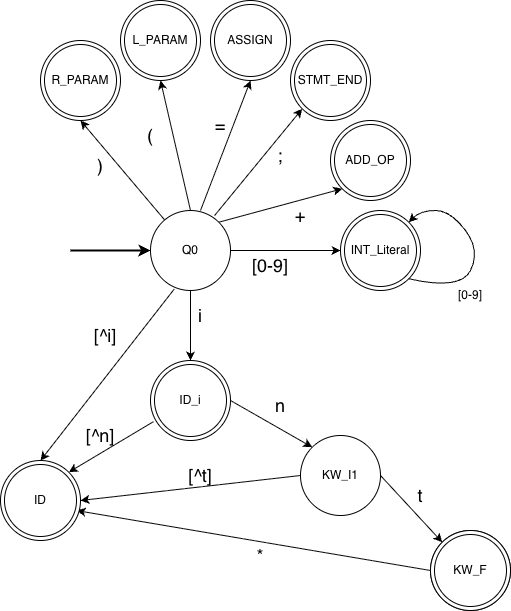
\includegraphics[width=0.45\textwidth]{lexerDFA.png}
    \caption{If a state receives an input for which there is no transition it's considered to go to a trap state}
\end{figure}


This DFA is implemented using a 2D array where rows represents the state and the columns represents the possible input character types and transitions between states can be as simple as,
\begin{verbatim}
    new_state = transition_table[current_state][input_char_type];
\end{verbatim}

This lexer implementation returns the matching token thus it can be feed into the next stage of the pipeline without storing the entire token stream in memory

\subsection{Parser}

With the pipeline design of the lexer a bottom up parser would be the most optimal and efficient design but due to the size of the grammar the manual creation of a the tables didn't seem feasible thus a \textbf{recursive descent parser} was implemented in the file (\texttt{parser.c}).

\subsubsection{Limitations of the Parser}
\begin{itemize}
    \item \textbf{Issue:} Since this is a recursive descent parser the grammar had to be right recursive thus would make the associativity of the operators incorrect.

    \item \textbf{Solution:} To solve this i've implemented the recursive rules with iteration instead of recursion thus the associativity is maintained even though only the plus operator was needed for this assignment.

\end{itemize}

The parser then finally uses the convenience functions defined in the file (\texttt{parseTree.c}) to create the parse tree which is then used by the executor

\subsection{Executor}

The executor is implemented in the file (\texttt{executor.c}) and it uses a symbol table implemented in the file (\texttt{symbolTable.c}) to store the variables and their values. The executor traverses the parse tree and executes the program by evaluating the expressions and updating the symbol table accordingly.

\section{Usage and Testing}

Even though this was asked to build using just a single file due to the modular implementation and out-scope features i've implemented the compiler using multiple files. 

I've attached a pre-processor compiled version of the code in a songle file named (\texttt{compiler.c}) which can be used but for referencing the code please refer to the individual files in the source code folder.

To compile the code in the source code folder you can simply run the command,
\begin{verbatim}
    make
\end{verbatim}

This will create an executable named \texttt{a.out} which can be run using the command,
\begin{verbatim}
    ./a.out <input_file> -i -d <delay_in_ms>
\end{verbatim}

The arguments are as follows,
\begin{itemize}
    \item \texttt{<input\_file>} - The file containing the source code to be executed
    \item \texttt{-i} - when this flag is used the compiler will pase at each token read and wait for the user to press enter before continuing this is useful for debugging and understanding the flow of the compiler and the creation of the parse tree
    \item \texttt{-d <delay\_in\_ms>} - This flag is used to slow down the execution of the compiler by adding a delay between each token read. Cannot be used with the \texttt{-i} flag
\end{itemize}

\end{document}
